\chapter{Design}

The design of Snapstore had two steps. The first was to identify the purposes of a VCS. The second was to create a conceptual model composed of concepts that fulfilled the purposes of a VCS.

\section{Purposes of Version Control}

The six purposes of a VCS identified in \cite{RossoJackson} were used in the design of Snapstore. A purpose graph showing these purposes in the context of Snapstore is included in Figure 3-1, where each sub-purpose points to its parent purpose. A purpose is a sub-purpose of another purpose if it supplements it. The purposes are classified into five categories: data management, change management, collaboration, parallel development, and disconnected operation.

\begin{figure}
\begin{center}

\includegraphics[max width= \linewidth]{PurposeGraph}
\end{center}
\caption{Purpose Graph of Version Control Systems.}
\label{arm:fig1}
\end{figure}

\textbf{Data Management} deals with the notion of backup. In case of failure, data needs to be stored persistently and be able to be retrieved. This purpose class addresses risks associated with development such as accidental deletion and incorrect saves, in addition to machine failure. The ability to track and untrack files gives the user control over what files will be persistently stored.

The second class, \textbf{change management}, deals with managing edits. Grouping changes allows the user to divide the history of a file or files in logical segments. Groups allow users to create segments in their projects and file histories. Tagging these groups as coherent points in development aid in administrative and managerial tasks associated with complex projects. These coherent points in the project can then be returned to by reverting the project to reflect the versions of files in that group.

\textbf{Collaboration} concerns a project shared by multiple users. Synchronizing the changes of collaborators on that system amalgamates their edits and distributes them in such a way that every collaborator can agree on the nature and ordering of the changes.

\textbf{Parallel Development}, the fourth class, deals with supporting parallel lines of development. Switching between parallel lines, as well as merging parallel lines are both needed to fully support parallel development. Merging must be done in a way that prevents conflicts when possible and makes them explicit when they cannot be avoided. This purpose allows users more flexibility to isolate parts of their work from others and to develop without affecting the main line.

The final class, \textbf{Disconnected Operation}, allows operations to be performed in a disconnected mode. Any work that a user can do in the VCS should be possible in an offline setting or in a setting where the user has willingly disconnected from their collaborators.

\section{Conceptual Model}

Once the purposes of VCSs were defined, a conceptual model that addressed those purposes and that was aligned with conceptual design theory \cite{Jackson} was created. A mapping of each Snapstore concept to its motivating purpose is shown in Table 3.1. Table 3.2 shows each Snapstore concept and its operational principle. A graphical representation of the conceptual model, using the notation for extended entity-relationship diagrams as used in \cite{SantiagoJackson}, is shown in Figure 3-2.

\begin{table}
\begin{tabular}{ |p{3cm}||p{5cm}||p{7cm}|}
 \hline
 \textbf{Purpose Class} & \textbf{Concept} & \textbf{Motivating Purpose}\\[8pt]
 \hline
 \parbox[t]{3cm}{Data \par Management\strut} & Snapshot & Make a set of changes to a file persistent\\[8pt]
 %
  & Snapstore Folder & Provide a platform for users to edit files\\[8pt]
 %
  & Tracked File & Mark files whose changes should be saved\\[8pt]
 %
  & Untracked File & Mark files whose changes should be ignored\\[8pt]
 \hline
 \parbox[t]{3cm}{Change \par Management\strut} & Group & Group logically related changes together\\[8pt]
  & Tag & Represent and record coherent points in history\\[8pt]
 \hline
 Collaboration & Upstream Repository & Synchronize changes of collaborators\\[8pt]
 \hline
 \parbox[t]{3cm}{Support \par Parallel Lines\strut} & Branch & Support parallel lines of work\\[8pt]
  & Conflict Snapshot & Mark snapshots with unresolved conflicts\\[8pt]
 \hline
 \parbox[t]{3cm}{Disconnected \par Operation\strut} & Local Repository & Perform operations in disconnected mode\\[8pt]
 \hline
\end{tabular}
\caption{Concepts of Snapstore and their motivating purposes.}
\end{table}

\begin{table}
\begin{tabular}{ |p{2.25cm}||p{2.25cm}||p{12.5cm}|}
 \hline
 \textbf{Purpose Class} & \textbf{Concept} & \textbf{Operational Principle}\\[8pt]
 \hline
 \parbox[t]{3cm}{Data \par Management\strut} & Snapshot & Whenever a user saves a tracked file to disk from within the Snapstore Folder, a snapshot containing that file's contents is created and permanently stored in the snapshot graph for that file. The user can revert the file to a previous snapshot by navigating this snapshot graph and finding the correct snapshot. When the user reverts the file to this snapshot, the file's contents are modified to match the contents of the file at the point in time in which the snapshot was taken.\\[8pt]
 %
  & \parbox[t]{3cm}{Snapstore \par Folder\strut} & The user can see every file accessible to Snapstore by looking in the Snapstore folder. There, users can change the tracking status of those files and edit those files to create new snapshots.\\[8pt]
 %
  & \parbox[t]{3cm}{Tracked \par File\strut} & By making a file tracked, the user causes snapshots to be made of that file whenever edits of that file are saved to disk. These snapshots are stored in the local and upstream repository, and collaborators on the branch in which those snapshots were created can see them.\\[8pt]
 %
  & \parbox[t]{3cm}{Untracked \par File\strut} & The user can cause snapshots to stop being created for a file by making it an untracked file. Untracked files will not be saved in the local or upstream repository, and collaborators cannot see changes made to untracked files.\\[8pt]
 \hline
 \parbox[t]{3cm}{Change \par Management\strut} & Group & A user can place logically related snapshots in a group to increase the organization of their branch. The user can view this group by searching for its group name, and all collaborators on that branch can do the same.\\[8pt]
  & Tag & When a user places a tag on a group, it becomes findable by that tag's name in addition to the group name. This tag is also shared with all collaborators of that user. When the user reverts this tagged group, every file in that group is reverted to their snapshot in that group.\\[8pt]
 \hline
 Collaboration & \parbox[t]{3cm}{Upstream \par Repository\strut} & Whenever a user makes a change on a branch that other users have access to, that change is propagated by the upstream to those other users. Upstreams synchronize the changes made by collaborators so that each local repository has the same data.\\[8pt]
 \hline
 \parbox[t]{3cm}{Support \par Parallel Lines\strut} & Branch & When the user switches branches, Snapstore hides the old branch's data, shows them the current branch's data, and allows them to start adding data to the current branch. Branches separate data on independent lines of development for the user.\\[8pt]
  & \parbox[t]{3cm}{Conflict \par Snapshot\strut} & When the merge of two snapshots results in a conflict, a conflict snapshot is created. This conflict snapshot shows the user where the conflict exists using conflict markers. Fixing the conflict creates a new snapshot.\\[8pt]
 \hline
 \parbox[t]{3cm}{Disconnected \par Operation\strut} & \parbox[t]{3cm}{Local \par Repository\strut} & All saved changes made by the user are first stored persistently in the local repository, allowing them to work offline. When a network connection is restored, the local repository will push any data created while offline to the connected upstream.\\[8pt]
 \hline
\end{tabular}
\caption{Concepts of Snapstore and their operational principles.}
\end{table}


\begin{figure}
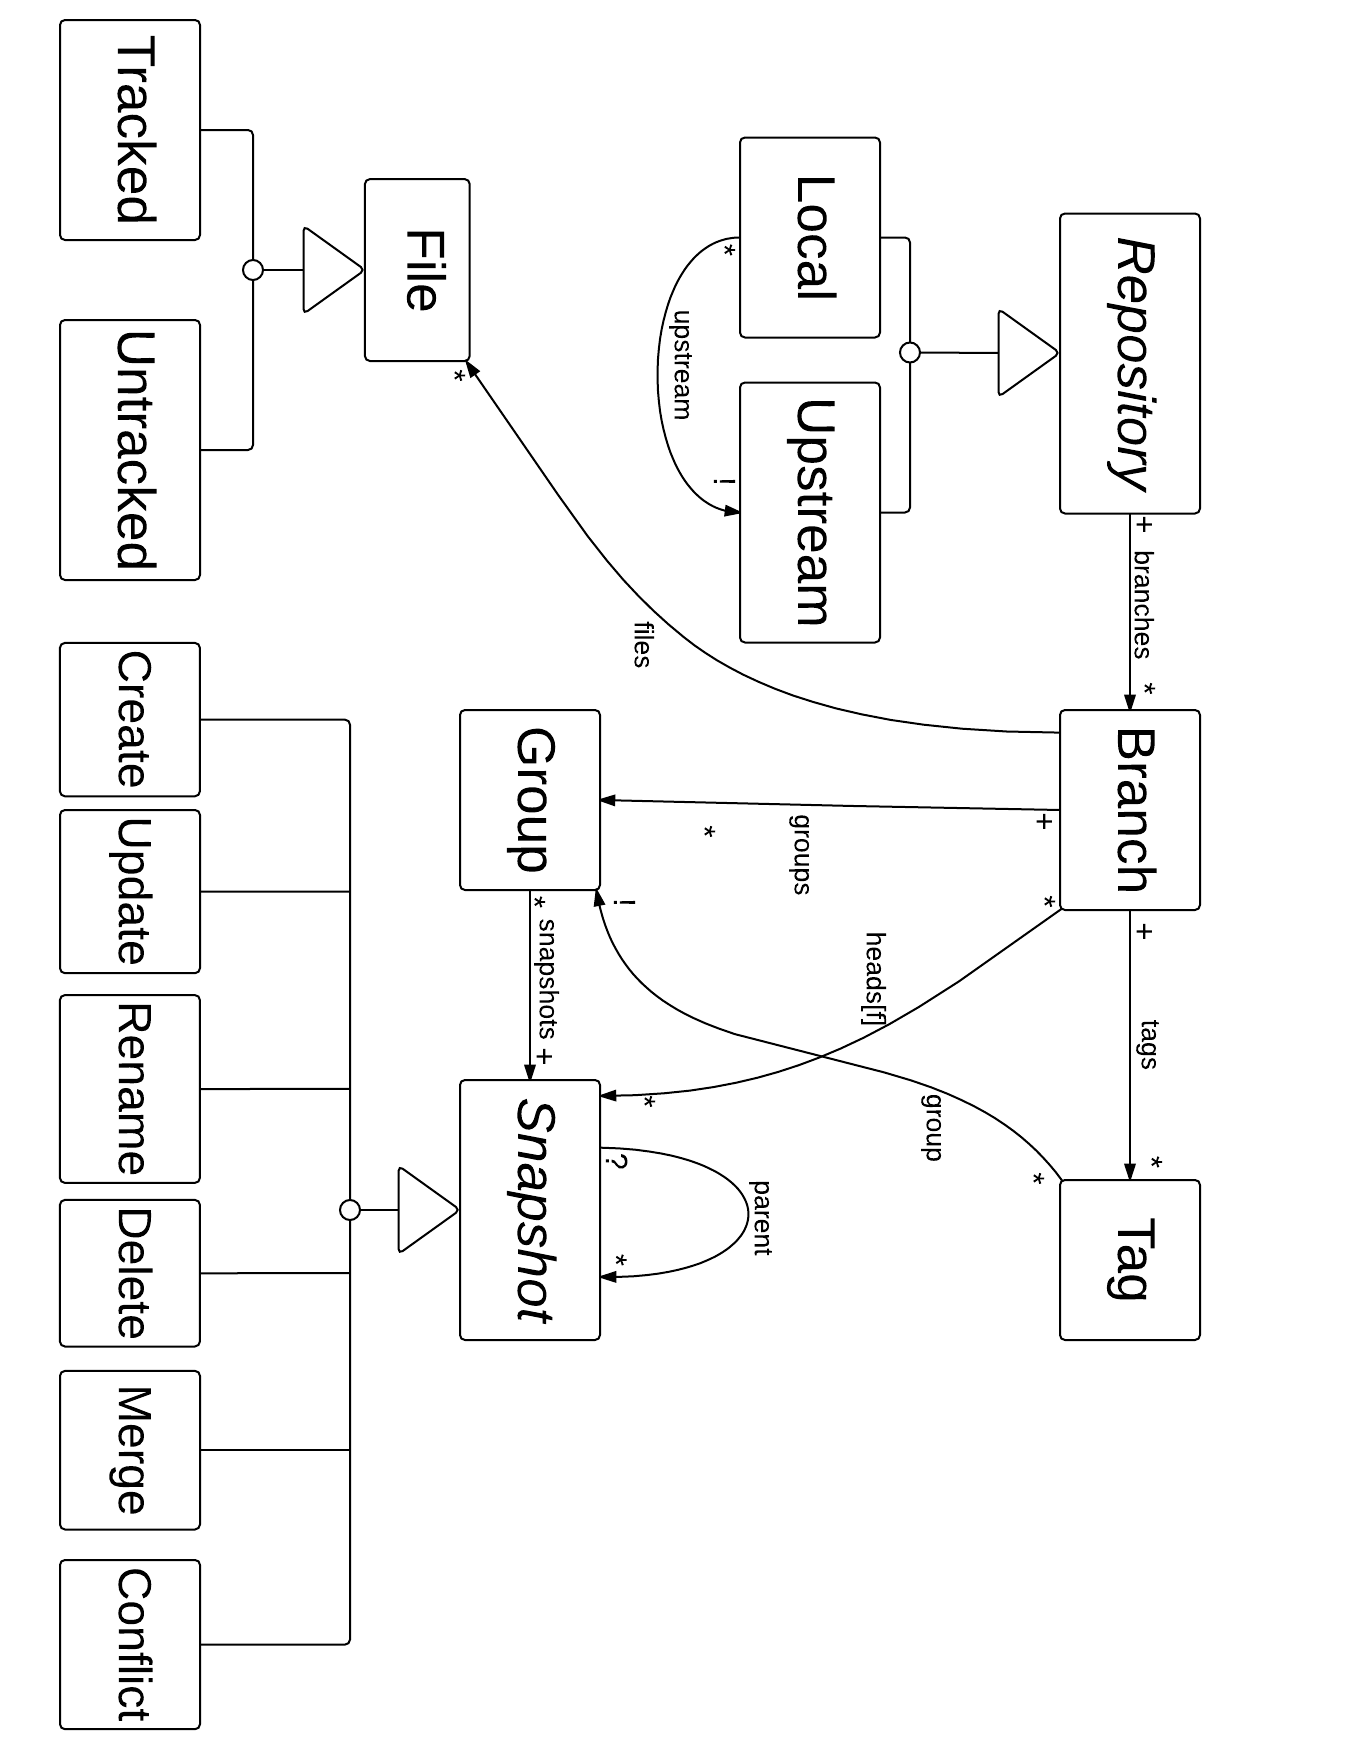
\includegraphics[max width= \linewidth]{ConceptModel}
\caption{Concept Model of Snapstore.}
\label{arm:fig1}
\end{figure}

\subsection{Data Storage --- Snapshot}

Persistent data storage in Snapstore is achieved with the notion of a \textit{snapshot}. A snapshot is a saved state of a file. Snapshots record updates, renames, moves, deletes, along with merges and conflicts. The \textit{head} snapshot for any given file is the most recent snapshot made for that file and reflects the current content of that file on disk. 

The type of snapshot dictates the values of that snapshot's attributes. Create snapshots\footnote{Create snapshots are a type of snapshot. The identifier ``create'' is not an action. Rather, it refers to the fact that this snapshot was made when a file was first created. Create snapshots represent the \textit{root} of a file's snapshot graph.} have no parent. Update snapshots have a parent, a child, and content. Rename snapshots have a different file name than their parent. Delete snapshots have no content, though they still have a parent and can therefore be placed in the snapshot graph. Merge snapshots have more than one parent, and conflict snapshots are merge snapshots that have conflict markers in their data.

The snapshots of a file are related by the graph they create with their parent/child relationships. This ordering forms the snapshot graph described in section 2.1.1. Each unique (branch, file) tuple is represented by its own snapshot graph.

The snapshot graph is guaranteed to be an in-order description of snapshots a specific client has made to a file in a branch. There is no operation on the client that distorts the ordering of snapshots in the graph. The only operation that can alter the graph occurs when another client's snapshot is inserted in the graph. This can occur when two users are on a shared branch and they need to share snapshots. However, even if snapshots are inserted into a user's snapshot graph, the user's ordering of locally made snapshots stays intact.

Any file, identified by its snapshot graph, can either be tracked or untracked. Edits made to untracked files will not result in the creation of new snapshots.

\subsection{Grouping Changes --- Group}

A \textit{group} is a collection of logically related snapshots, identified by a group name. A group must contain at least one snapshot, but there are no restrictions on what kinds of snapshots can be in the group or what their relationship must be. The same snapshot can exist in more than one group. It is up to the user to decide what makes a group of snapshots logically related. This allows flexibility in projects and development strategy.

Groups are an attribute of a specific branch. Even if two groups contain the same snapshots across different branches, those groups are different because they exist on different lines of development.

\subsection{Recording Coherent Points --- Tag}

The notion of a \textit{tag} allows users to label logical milestones in their work. They describe a group but have an added function over a group's name: they describe the status of the group as representing a coherent point. Here, coherent means that the project is in a state that is ready for further development or work, though this definition may differ from project to project \cite{RossoJackson}. 

Tags will always describe groups that are perfectly vertical. A perfectly vertical group is one with at most one snapshot from any file. An example of this is tagging a group containing every head snapshot in a branch with the tag ``Submitted to Scientific Journal'' or ``Version 1.0''.

Tags are also an attribute of the branch. This means that they are created inside of an independent line of development. They can be copied across branches when merging and cloning, but they stay an attribute of the branch.

\subsection{Support Parallel Lines --- Branch}

In Snapstore, the \textit{branch} supports parallel and independent lines of development. These branches are completely separate from each other and facilitate the partitioning of data. The branch houses three of the other main concepts in Snapstore: snapshots, groups, and tags. These three concepts together constitute a line of development, and so the branch is the conceptual representation of that line.

Branches can be shared between multiple users. Users on a shared branch can make changes to the snapshots, groups, and tags of that branch, and the other collaborators will receive those changes. We have opted to use a last-write-wins approach when dealing with conflicts on a shared branch because it is an easier paradigm for non-technical users to understand compared with merging. Plus, with the potential amount of conflicts on a shared branch, the number of merges would be very high. Because of this, merging is only done between branches on the local repository.

This approach can result in a snapshot being very far removed from its original parent. For example, say Alice and Bob share a branch with a single snapshot. Alice goes offline and makes one snapshot of her own. Bob, still online, makes 10 snapshots that are immediately confirmed by the server. When Alice returns to the network, her snapshot would be placed after Bob's 10 confirmed snapshots, far from its original parent.

Despite this, we believe this approach is appropriate for two reasons. First, in the highly connected environment of today's computing, making that many offline edits is typically done by choice. Second, if the user knows that offline edits will be an issue, Snapstore allows them to create a separate branch for highly disconnected development. Users can create a separate branch they can work on offline, and they can merge back into the main branch when they're finished.

Branches can also be merged together, synchronizing the parallel development. This involves combining each branch's individual snapshot, group, and tag data, as explained in section 2.2.3.

\subsection{Synchronize Changes of Collaborators --- Upstream Repository}

Snapstore uses a centralized data storage system called an \textit{upstream repository}, or upstream, to synchronize the data of collaborators. When multiple users share a branch, their data is shared via the upstream, synchronizing all local repositories.

When one collaborator makes a change at the branch level (branches, snapshots, groups, tags), it is reflected in the upstream. The upstream then searches for other collaborators on that branch and pushes the change down to them.

Every local repository can have one upstream, though it does not have to be the default Snapstore upstream. This allows the user to choose the location through which their data passes.

\subsection{Disconnected Operation --- Local Repository}

The ability to leverage the benefits of a VCS without needing an Internet or network connection is enabled by the \textit{local repository}. The local repository holds all of the branch, snapshot, group, and tag data for a user.

When any data is saved by the user, it is first saved to the local repository, whether or not there is network connection. This allows users to operate Snapstore offline, with all functionality except sharing. When a network connection is restored after a period of disconnected development, all of the local data created in the interim is pushed to the upstream.

\subsection{Discussion}

During the design process, there were many decisions made that had lasting tradeoffs for Snapstore. The main tradeoffs are explored below.

\subsubsection{Granularity of a Snapshot}

The decision of what a snapshot should represent was the first design decision we encountered. Either a snapshot could represent the state of a file, or it could represent the state of every file in a branch. 

The first reason we decided to make the snapshot describe the state of a single file was that it was more intuitive to a typical user. If a user was to save a file and create a snapshot, they would expect that snapshot to relate to the object they just interacted with, that file. They would not expect it to relate to every file in the branch.

Another reason for this decision was the necessity of the group concept. In many VCSs, such as Git, saving changes couples together the act of saving changes with the act of grouping changes (a git commit), resulting in an overloaded concept \cite{Jackson}. If a snapshot represented the state of every file in a branch, then it could also be a group. We designed the snapshot to represent the state of a single file to conceptually separate the saving of changes with the grouping of those changes.

\subsubsection{The Upstream}

Different VCSs and file syncing systems have different storage models. Git, for example, uses a decentralized storage system. Dropbox and SVN, on the other hand, use a centralized system. When deciding which model to use for our upstream, we looked at both models' pros and cons. Centralized VCSs are easier to learn and use \cite{Brindescu}, but they require an Internet connection for all operations other than file edits and don't allow users to share directly with each other. Decentralized VCSs do allow users to work offline and share with each other, but they also have more space requirements because the version history for every file exists on every machine.

Snapstore uses a hybrid centralized/decentralized upstream model. On one hand, it is centralized because all collaboration takes place via the upstream repository. Any data a user wants to collaborate on with another user must go through the upstream first. On the other hand, Snapstore is also decentralized because users have a local repository, where actions can be made without a network connection. Snapstore users have all of their data on their own machine, just like in a decentralized VCS. Users can work offline, without checking out a central repository.

There are downsides to this hybrid model. Because Snapstore local repositories can only have one upstream, shared data will always be controlled by a single, centralized entity. And, this upstream must always be online in order to facilitate collaboration. Users also cannot share directly with a subset of collaborators on a shared branch. They can, however, work around this limitation by creating a new branch with that subset of users.

Despite these downsides, we believe this hybrid model is a good balance between the centralized and decentralized models. The centralized characteristics make it easier to learn and use, and the decentralized characteristics make it more powerful.

\subsubsection{File Names}

Whether to make the file name a property of the file or the identifier for the file was an important decision for Snapstore. Git, for example, uses the file's name as its identifier. Because of this decision, renames to a file are sometimes processed as deleting that file and creating a new file, causing much consternation among users, especially novices \cite{RossoJackson}.

We wanted to robustly support renaming files in Snapstore, so file names in Snapstore are simply a property of the file. Each snapshot in a given snapshot graph will have the same file id. When branch merging occurs, only snapshot graphs with the same file id will be merged. The merge operation will search the file's two snapshot graphs for a common ancestor and perform a three-way merge. This allows Snapstore to accurately handle renames and merges.



